\documentclass[aspectratio=43,11pt]{beamer}
\usepackage{amsmath,amssymb,graphicx,listings,lmodern,
            xcolor,booktabs,array,soul, calc}
\usetheme{default}
\usecolortheme{default}
\definecolor{aggiemaroon}{RGB}{80,0,0}
\setbeamercolor{structure}{fg=aggiemaroon}
\setbeamertemplate{navigation symbols}{}
\setbeamertemplate{footline}[frame number]
\setbeamertemplate{itemize items}[circle]

\usepackage{tikz,pgfplots}
\pgfplotsset{compat=1.18}
\definecolor{darkred}{RGB}{90,0,0}
\definecolor{plotblue}{RGB}{35,85,155}
\definecolor{plotorange}{RGB}{225,155,75}
\definecolor{overlapgreen}{RGB}{100,160,125}

\usepackage[T1]{fontenc}
\newcommand{\MI}{I(X;Y)}
\newcommand{\Hb}{H_{\mathrm b}}
\title{Decision and Risk Analysis}
\subtitle{Lecture 9: \textbf{Mutual Information\\}(not in the textbook!)}
\author{}
\date{\color{aggiemaroon}{DAEN 427 / ISEN 427 / ISEN 627 - Fall 2026\\
      \textbf{Alexander Abuabara}}}
\titlegraphic{\vfill 
\includegraphics[height=1.2cm]{TAMU_logo.png}}

\begin{document}

\begin{frame}
\titlepage
\end{frame}

\begin{frame}{Question}
Suppose we observe two variables:
\begin{itemize}
\item $X$: weather (rainy or sunny)
\item $Y$: whether a person carries an umbrella (yes or no)
\end{itemize}
\vspace{0.5em}
How much does observing $X$ reduce our uncertainty about $Y$?
\begin{block}{Mutual information}
Measures \emph{statistical dependence} rather than just a linear association.
\end{block}
\end{frame}

\begin{frame}{Example: 100 observations}
\centering
\begin{tabular}{lrrr}
\toprule
& Umbrella: yes & Umbrella: no & Total\\
\midrule
Rainy & 40 & 10 & 50\\
Sunny & 10 & 40 & 50\\
\midrule
Total & 50 & 50 & 100\\
\bottomrule
\end{tabular}
\vspace{1em}
\begin{itemize}
\item $P(Y=\text{yes})=50/100=0.5$.
\item $P(Y=\text{yes}\mid X=\text{rainy})=40/50=0.8$.
\item $P(Y=\text{yes}\mid X=\text{sunny})=10/50=0.2$.
\end{itemize}
\medskip
The weather is informative, but not perfectly predictive.
\end{frame}

\begin{frame}{Probability terms}
\begin{description}
\item[Marginal] $p(y)$: chance of an umbrella, ignoring weather.
\item[Joint] $p(x,y)$: chance of a particular weather--umbrella pair.
\item[Conditional] $p(y\mid x)=p(x,y)/p(x)$: chance of an umbrella after weather is known.
\item[Independence] $p(x,y)=p(x)p(y)$ for every pair $(x,y)$.
\end{description}
\medskip
For example:
\[
p(\text{rainy, yes})=0.40,\qquad
p(\text{yes}\mid\text{rainy})=\frac{0.40}{0.50}=0.80.
\]
\end{frame}

\begin{frame}{What is information?}
Less likely events carry more \ul{information} because they reduce our uncertainty more when they occur.\\
\medskip
Consider two events:
\begin{itemize}
\item Event A: The sun rises tomorrow. Probability is nearly 1.
\item[\rightarrow] If Event A occurs, you learn almost nothing new because you already expected it.\\
\item Event B: You win a lottery with a one-in-a-million chance.
\item[\rightarrow] If Event B occurs, you learn something highly unexpected. The observation rules out a much larger set of possibilities.\\
\end{itemize}
\medskip
Thus, \hl{the less predictable} an event is,\\\hl{the more information} its occurrence provides.
\end{frame}

\begin{frame}{What is information in bits?}
The \emph{surprisal} of an event with probability $p$ is
\[
\mathcal I(\text{event})=-\log_2 p\quad\text{bits}.
\]
\begin{itemize}
\item Probability $1/2$ $\rightarrow$ $1$ bit of surprisal.
\item Probability $1/4$ $\rightarrow$ $2$ bits of surprisal.
\item Probability $1$ $\rightarrow$ $0$ bits of surprisal.
\end{itemize}
\medskip
A less likely event is more surprising.\\
A base-2 logarithm expresses information in \emph{bits}.
\end{frame}

\begin{frame}[t]{}
\vfill
\small
The \emph{surprisal} of an event with probability $p$ is
$\boxed{\mathcal{I}(p)=-\log_2 p \quad \text{bits}}$

\begin{columns}[T,onlytextwidth]

% LEFT COLUMN
\begin{column}{0.4\textwidth}
\vspace{0.55cm}
\textbf{Examples:}
\vspace{0.25cm}
\begin{itemize}
    \setlength{\itemsep}{0.35cm}

    \item[$\color{darkred}\bullet$]
    $p=\frac12 \Rightarrow 1$ bit

    \item[$\color{darkred}\bullet$]
    $p=\frac14 \Rightarrow 2$ bits

    \item[$\color{darkred}\bullet$]
    $p=1 \Rightarrow 0$ bits
\end{itemize}
\end{column}

% RIGHT COLUMN
\begin{column}{0.6\textwidth}
\centering
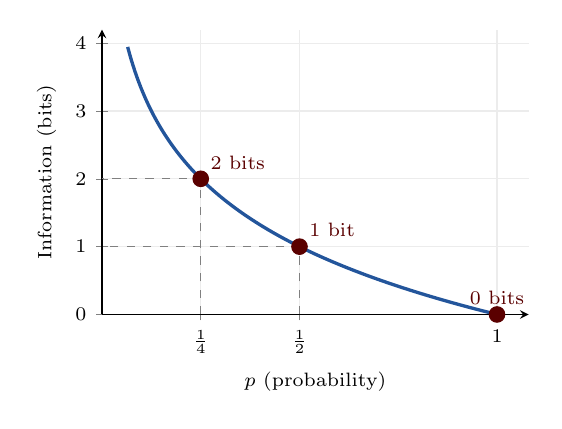
\begin{tikzpicture}
\begin{axis}[
    width=7.0cm,
    height=5.2cm,
    xmin=0, xmax=1.08,
    ymin=0, ymax=4.2,
    xlabel={$p$ (probability)},
    ylabel={Information (bits)},
    xlabel style={font=\scriptsize},
    ylabel style={font=\scriptsize},
    tick label style={font=\scriptsize},
    xtick={0.25,0.5,1},
    xticklabels={$\frac14$,$\frac12$,$1$},
    ytick={0,1,2,3,4},
    axis lines=left,
    grid=major,
    grid style={gray!15},
    clip=false
]
% Surprisal curve
\addplot[
    plotblue,
    very thick,
    domain=0.065:1,
    samples=200
] {-ln(x)/ln(2)};
% Dashed guides
\draw[dashed,gray]
    (axis cs:0.25,0) -- (axis cs:0.25,2)
    -- (axis cs:0,2);

\draw[dashed,gray]
    (axis cs:0.5,0) -- (axis cs:0.5,1)
    -- (axis cs:0,1);
% Highlighted points
\addplot[
    only marks,
    mark=*,
    mark size=2.8pt,
    darkred
] coordinates {
    (0.25,2)
    (0.5,1)
    (1,0)
};
% Labels
\node[above right,font=\scriptsize,darkred]
    at (axis cs:0.25,2) {2 bits};

\node[above right,font=\scriptsize,darkred]
    at (axis cs:0.5,1) {1 bit};

\node[above,font=\scriptsize,darkred]
    at (axis cs:1,0) {0 bits};
\end{axis}
\end{tikzpicture}
\end{column}
\end{columns}
\begin{beamercolorbox}[
    wd=\textwidth,
    sep=7pt,
    center
]{normal text}
Less likely events carry more information.
\end{beamercolorbox}
\end{frame}

\begin{frame}{What Is Entropy?}
\small
Entropy is a foundational concept in physics that measures the dispersal of energy, randomness, or disorder within a closed system.\\
\medskip
Here, entropy measures the average uncertainty associated with a random variable.
\begin{itemize}
  \item \textbf{High entropy:} outcomes are difficult to predict.
  \item \textbf{Low entropy:} outcomes are easier to predict.
  \item \textbf{Zero entropy:} the outcome is certain.
\end{itemize}
\[
H(X)=-\sum_x P(x)\log_2 P(x)
\]
\vspace{-0.75em}
\begin{center}
\small
\begin{tabular}{lcc}
\toprule
\textbf{Coin toss} & \textbf{$P(\text{Heads})$} & \textbf{Entropy} \\
\midrule
Fair coin & $0.50$ & $1.000$ bit \\
Biased coin & $0.90$ & $0.469$ bits \\
Certain heads & $1.00$ & $0$ bits \\
\bottomrule
\end{tabular}
\end{center}
{More uncertainty before observing the outcome means more information gained when it is revealed, on average.}
\end{frame}

\begin{frame}{Entropy: average uncertainty}
For a discrete random variable $Y$,
\[
H(Y)=-\sum_y p(y)\log_2 p(y).
\]
\begin{itemize}
\item Entropy is the \emph{expected surprisal} before observing $Y$.
\item By convention, $0\log_2 0=0$.
\item For two equally likely outcomes, entropy is $1$ bit.
\end{itemize}
In our example, umbrella use is evenly split:
\[
H(Y)=-0.5\log_2 0.5-0.5\log_2 0.5=\boxed{1\text{ bit}}.
\]
\end{frame}

\begin{frame}{Conditional entropy: uncertainty after $X$}
\small
\[
H(Y\mid X)=\sum_x p(x)H(Y\mid X=x),
\]
where
\[
H(Y\mid X=x)=-\sum_y p(y\mid x)\log_2 p(y\mid x).
\]
Rainy days: $80\%$ carry umbrellas, $20\%$ do not:
\[
H(Y\mid\text{rainy})=-0.8\log_2 0.8-0.2\log_2 0.2
\approx 0.722.
\]
Sunny days have the probabilities reversed, so the entropy is also $0.722$.
\[
H(Y\mid X)=0.5(0.722)+0.5(0.722)=\boxed{0.722\text{ bits}}.
\]
\end{frame}

\begin{frame}{Mutual information (reduction)}
\[
\boxed{I(X;Y)=H(Y)-H(Y\mid X)}
\]
For the weather--umbrella data:
\[
I(X;Y)=1-0.722=\boxed{0.278\text{ bits}}.
\]
\begin{itemize}
\item Knowing the weather removes, on average, $0.278$ bits of the original $1$ bit of uncertainty about umbrella use.
\item Here this is a $27.8\%$ reduction \emph{because} the initial entropy is exactly $1$ bit.
\item MI is not generally a percentage.
\end{itemize}
\end{frame}

\begin{frame}{The joint-probability formula}
An equivalent definition is
\[
\boxed{I(X;Y)=\sum_{x,y}p(x,y)\log_2\frac{p(x,y)}{p(x)p(y)}}.
\]
\small
For our $2\times2$ table, the joint probabilities are $0.4,0.1,0.1,0.4$; every product $p(x)p(y)$ equals $0.25$:
\begin{align*}
I(X;Y)&=2(0.4)\log_2\frac{0.4}{0.25}
+2(0.1)\log_2\frac{0.1}{0.25}\\
&\approx\boxed{0.278\text{ bits}}.
\end{align*}

This also equals the KL divergence $D_{\mathrm{KL}}(p(x,y)\,\|\,p(x)p(y))$.\\
\medskip
\tiny{Kullback-Leibler divergence measures how different one probability distribution is from another. Mutual information is a special case of KL divergence. \url{https://en.wikipedia.org/wiki/Kullback–Leibler_divergence}}
\end{frame}

\begin{frame}[t]{}
\small
\begin{center}
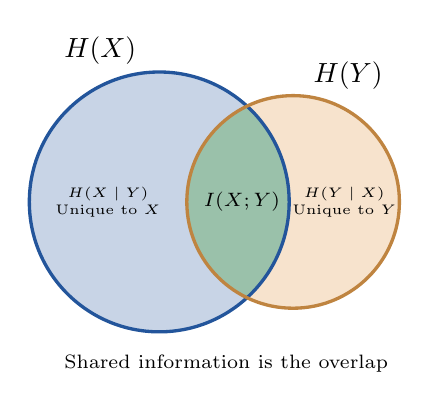
\begin{tikzpicture}[scale=1]
% Circle geometry
\def\radiusA{1.65}
\def\radiusB{1.35}
\coordinate (A) at (-0.85,0);
\coordinate (B) at (0.85,0);
% Entropy regions
\fill[plotblue!25] (A) circle (\radiusA);
\fill[plotorange!28] (B) circle (\radiusB);
% Overlapping region
\begin{scope}
    \clip (A) circle (\radiusA);
    \fill[overlapgreen!65]
        (B) circle (\radiusB);
\end{scope}
% Circle boundaries
\draw[plotblue,very thick]
    (A) circle (\radiusA);
\draw[plotorange!85!black,very thick]
    (B) circle (\radiusB);
% Labels outside circles
\node[font=\bfseries] at (-1.6,1.92) {$H(X)$};
\node[font=\bfseries] at (1.55,1.60) {$H(Y)$};
% Labels inside circles
\node[align=center,font=\tiny]
    at (-1.5,0)
    {$H(X\mid Y)$\\[0pt]Unique to $X$};
\node[align=center,font=\tiny]
    at (1.5,0)
    {$H(Y\mid X)$\\[0pt]Unique to $Y$};
\node[align=center,font=\scriptsize\bfseries]
    at (0.2,0)
    {$I(X;Y)$};
% Annotation
\node[font=\scriptsize,align=center]
    at (0,-2.05)
    {Shared information is the overlap};
\end{tikzpicture}
\end{center}
\vspace{-0.1cm}
\begin{center}
\begin{minipage}{0.975\textwidth}
\footnotesize
So, mutual information cannot exceed the entropy of either variable:
\[
\underbrace{
I(X;Y)=H(Y)-H(Y\mid X)
}_{\displaystyle \leq H(Y)}
\]
This means that knowing \(X\) cannot tell us more about \(Y\) than the total uncertainty in \(Y\), and vice versa.
\[
\boxed{
I(X;Y)\leq \min\{H(X),H(Y)\}
}
\]
\end{minipage}
\end{center}
\end{frame}

\begin{frame}{Important mathematical properties}
\begin{itemize}
\item \textbf{Nonnegative:} $I(X;Y)\geq 0$.
\item \textbf{Symmetric:} $I(X;Y)=I(Y;X)$.
\item \textbf{Zero exactly at independence:} $I(X;Y)=0$ if and only if $X$ and $Y$ are independent (for the true distribution).
\item \textbf{Upper bound for discrete variables:}
\[
I(X;Y)\leq\min\{H(X),H(Y)\}.
\]
\item \textbf{Perfect knowledge:} if $Y$ is fully determined by $X$, then $H(Y\mid X)=0$ and $I(X;Y)=H(Y)$.
\end{itemize}
\end{frame}

\begin{frame}{Mutual information vs. correlation}
\footnotesize
\begin{tabular}{p{0.12\linewidth}p{0.32\linewidth}p{0.46\linewidth}}
\toprule
& Pearson correlation $r$ & Mutual information $I$\\
\midrule
Captures & Linear association & Any statistical dependence\\ \hline
Sign & Negative, zero, positive & Nonnegative only\\ \hline
Scale & $-1$ to $1$ & $0$ to $\min(H(X),H(Y))$ {\tiny for discrete variables}\\ \hline
Units & Unitless & Bits {\tiny(base 2)} or nats {\tiny(natural log)}\\ \hline
Direction & Sign shows slope direction & No sign or causal direction\\
\bottomrule
\end{tabular}
\medskip
\begin{itemize}
\item Our binary weather--umbrella table has $\lvert r\rvert=0.60$ (with compatible $0/1$ coding), but $I=0.278$ bits.
\item They are \emph{different measures}, not numerically comparable.
\end{itemize}
\end{frame}

\begin{frame}{A nonlinear relationship correlation can miss}
Let $X$ be equally likely to be $-2,-1,0,1,2$, and let $Y=X^2$.
\[
\begin{array}{c|ccccc}
X & -2&-1&0&1&2\\\hline
Y &4&1&0&1&4
\end{array}
\]
\begin{itemize}
\item Pearson's $r=0$ because the positive and negative linear effects cancel.
\item But $Y$ is completely determined by $X$.
\end{itemize}
\end{frame}

\begin{frame}[t]{}
\footnotesize
Let $X$ be uniformly distributed over
$\{-2,-1,0,1,2\}$, with $Y=X^2$.\\
\medskip
\textbf{Step 1: Find the probability distribution of $Y$}
\begin{center}
\begin{tabular}{ccc}
\toprule
$Y$ & Corresponding $X$ & $P(Y=y)$ \\
\midrule
$0$ & $0$      & $\frac15$ \\
$1$ & $-1,1$   & $\frac25$ \\
$4$ & $-2,2$   & $\frac25$ \\
\bottomrule
\end{tabular}
\end{center}
\textbf{Step 2: Calculate the entropy of $Y$}
\[
H(Y)=-\sum_y P(y)\log_2 P(y)
\]
\[
H(Y) =-\frac15\log_2\frac15 -2\left(\frac25\log_2\frac25\right) \approx 1.522\ \text{bits}
\]
\textbf{Step 3: Calculate mutual information} {\tiny (next slide)} \\ % \textsuperscript
Since $Y=X^2$, knowing $X$ determines $Y$ exactly.
Therefore, $H(Y\mid X)=0$.
\[
\boxed{
I(X;Y)=H(Y)-H(Y\mid X)
      =1.522\ \text{bits}
}
\]
Knowing $X$ eliminates all uncertainty about $Y$.
\end{frame}

\begin{frame}[t]{}
\footnotesize
Let $X$ be uniformly distributed over $\{-2,-1,0,1,2\}$, with $Y=X^2$.\\
\smallskip
\textbf{Step 1: Examine the conditional probabilities}
\begin{center}
\begin{tabular}{ccc}
\toprule
Known $X$ & $Y=X^2$ & $P(Y=X^2\mid X)$ \\
\midrule
$-2$ & $4$ & $1$ \\
$-1$ & $1$ & $1$ \\
$0$  & $0$ & $1$ \\
$1$  & $1$ & $1$ \\
$2$  & $4$ & $1$ \\
\bottomrule
\end{tabular}
\end{center}
\smallskip
\textbf{Step 2: Calculate conditional entropy for each $X$}\\
For example, when $X=-2$, we know $Y=4$ with certainty:
\[
H(Y\mid X=-2)
=-1\log_2(1)=0.
\]
The same result holds for every other value of $X$.\\
\smallskip
\textbf{Step 3: Average over all possible values of $X$}
\[
H(Y\mid X) =\sum_x P(x)H(Y\mid X=x) =\frac15(0+0+0+0+0) = \boxed{0\text{ bits}}
\]
Since $Y=X^2$ is deterministic, knowing $X$ eliminates all uncertainty about $Y$.
\end{frame}

\begin{frame}[t]{}
\small
Recall that $X$ is uniformly distributed over $\{-2,-1,0,1,2\}$ and $Y=X^2$.\\
\medskip
\textbf{Entropy of $X$:}
\[
H(X)=\log_2 5\approx 2.322\text{ bits}
\]
\textbf{Mutual information:}
\[
I(X;Y)=H(Y)\approx 1.522\text{ bits}
\]
Knowing $X$ determines $Y$ exactly,\\
but knowing $Y$ does not always determine $X$.
\begin{center}
\begin{tabular}{ccc}
\toprule
Observed $Y$ & Possible $X$ & Remaining uncertainty \\
\midrule
$0$ & $0$       & $0$ bits \\
$1$ & $-1,1$    & $1$ bit \\
$4$ & $-2,2$    & $1$ bit \\
\bottomrule
\end{tabular}
\end{center}
\textbf{Remaining uncertainty about $X$:}
\[
\begin{aligned}
H(X\mid Y)
&=H(X)-I(X;Y)\\
&=2.322-1.522\\
&=\boxed{0.8\text{ bits}}
\end{aligned}
\]
The relationship is deterministic in one direction, but not invertible.
\end{frame}





\begin{frame}{A nonlinear relationship correlation can miss}
Let $X$ be equally likely to be $-2,-1,0,1,2$, and let $Y=X^2$.
\[
\begin{array}{c|ccccc}
X & -2&-1&0&1&2\\\hline
Y &4&1&0&1&4
\end{array}
\]
\begin{itemize}
\item Pearson's $r=0$ because the positive and negative linear effects cancel.
\item But $Y$ is completely determined by $X$.
\item $I(X;Y)=H(Y)$, probabilities of $Y=0,1,4$ are $1/5,2/5,2/5$.
\end{itemize}
\[
I(X;Y)=-\tfrac15\log_2\tfrac15-2\bigl(\tfrac25\log_2\tfrac25\bigr)
\approx\boxed{1.522\text{ bits}}.
\]
\end{frame}

\begin{frame}{Assumptions: theory vs. estimation}
\small
\textbf{Theoretical definition:}
\begin{itemize}
\item Requires a well-defined joint probability distribution.
\item Does \emph{not} require a linear relationship, Gaussian variables, or causality.
\item Formulas so far describe \emph{discrete} variables; continuous variables require probability densities and integrals.
\end{itemize}

\vspace{0.5em}
\textbf{Estimating MI from observations:}
\begin{itemize}
\item Observations should represent the target population or process.
\item The frequency-table estimator generally relies on sufficiently many observations in each relevant category.
\item Independence or an appropriate dependence-aware sampling model matters for uncertainty estimates and significance tests.
\end{itemize}
\end{frame}

\begin{frame}{Limitations and common pitfalls}
\small
\begin{itemize}
\item \textbf{Not causal:} MI cannot establish whether weather causes umbrella use, or vice versa.
\item \textbf{No direction or sign:} $I(X;Y)=I(Y;X)$; it cannot say whether a relationship increases or decreases.
\item \textbf{Finite-sample bias:} plug-in estimates are often positive even for truly independent variables.
\item \textbf{High dimensionality:} sparse counts and continuous-density estimation become difficult; binning choices affect results.
\item \textbf{No universal maximum:} raw MI depends on entropy and alphabet size, so values across different feature pairs may not be directly comparable.
\item \textbf{Redundant predictors:} a feature's MI with the target does not measure its additional value given other features.
\end{itemize}
\end{frame}

\begin{frame}{Does 1 information bit equal 1 computer bit?}
\textbf{Yes, in the unit of measurement:} both use base-2 logarithms.
\medskip
\begin{itemize}
\item A \textbf{binary digit} is a storage symbol, either 0 or 1.
\item A \textbf{Shannon bit} measures uncertainty or expected information.
\item An equally likely random 0/1 value has entropy $1$ bit.
\item A constant 0/1 value still occupies one binary digit if stored, but has entropy $0$ bits.
\end{itemize}
\medskip
\begin{block}{Connection to \hl{compression}}
For ideal lossless coding of long sequences, entropy in bits per symbol gives a fundamental lower limit on \emph{average} coding rate (under appropriate source assumptions). Actual storage also reflects coding overhead and representation.
\end{block}
\end{frame}

\begin{frame}{Putting the ``bit'' interpretation together}
\begin{itemize}
\item Before weather: umbrella use is a balanced yes/no question $\rightarrow H(Y)=1$ bit.
\item After weather: uncertainty averages $0.722$ bits.
\item The gain from weather is $0.278$ bits on average.
\end{itemize}
\medskip
\[
\underbrace{1}_{\text{before}}
=\underbrace{0.278}_{\text{information gained}}
+\underbrace{0.722}_{\text{uncertainty left}}
\quad\text{bits}.
\]\\
\medskip
This does \emph{not} mean that each weather observation physically stores $0.278$ of a binary digit. It is an \emph{average reduction in uncertainty}.
\end{frame}

\begin{frame}{}
\begin{enumerate}
\item Entropy is average uncertainty;\\
      conditional entropy is uncertainty remaining after observing another variable.
\item Mutual information is their difference,\\
      or equivalently the divergence between the joint distribution and independence.
\item MI detects nonlinear dependence that Pearson correlation can miss.
\item MI is noncausal and sensitive to how probabilities are estimated from finite data.
\item One Shannon bit uses the same mathematical unit as a digital bit, \ul{but} information content is not the same thing as a physical storage location.
\end{enumerate}
\end{frame}

\end{document}